%\documentclass[floatfix,prb,aps,superscriptaddress,11pt,preprint,letterpaper]{revtex4}
%\usepackage{amsfonts}
%\usepackage{amsmath}
%\usepackage{graphicx}
%\allowdisplaybreaks[1]%biutiful equation breaker!!!
%\usepackage{ulem}
%\usepackage{subfigure}
%\usepackage{fancyvrb}
%\usepackage{bm}
%%%%%*****************%%%% fine hyperef 
%\usepackage[backref,pdffitwindow,colorlinks,linkcolor={blue},citecolor={red}]{hyperref}
%%%%%%%%%%%%%%%%%%%%%%%%%%%%%%%%%%%%%%%%
%%\usepackage{showlabels}
%%\usepackage{showkeys}



\chapter{Theory}\label{ch:theory}

\section{Introduction}\label{intro}

Second harmonic generation (SHG) is a powerful spectroscopic tool for 
studying the optical properties of surfaces and interfaces since it has 
the advantage of being surface sensitive. Within the dipole approximation, 
inversion symmetry forbids SHG from the bulk of controsymmetric materials. 
SHG is allowed at the surface of these materials where the inversion symmetry 
is broken and should necessarily come from the localized surface region. 
SHG allows the study of the structural atomic arrangement and phase 
transitions of clean and adsorbate covered surfaces. Since it is also an 
optical probe it can be used out of UHV conditions and is non-invasive 
and non-destructive. Experimentally, new tunable high intensity laser systems 
have made SHG spectroscopy readily accessible and applicable to a wide range 
of systems.\cite{downer_optical_2001,lupke_characterization_1999}

However, theoretical development of the field is still an ongoing 
subject of research. Some recent advances for the cases of semiconducting 
and metallic systems have appeared in the literature, where the use of 
theoretical models with experimental results have yielded correct 
physical interpretations for observed SHG spectra.
\cite{
downer_optical_2001,
mendoza_ab_2001,
lim_optical_2000,
gavrilenko_optical_2000,
mendoza_visible-infrared_1999,
mendozaPRL98,
mendozaPRB96,
mendoza_polarizable-bond_1997,
guyotPRB90} 

In a previous article\cite{mendoza_epioptics_2001} we reviewed some 
of the recent results in the study of SHG using the velocity gauge 
for the coupling between the electromagnetic field and the electron. 
In particular, we demonstrated a method to systematically analyze the 
different contributions to the observed SHG peaks.\cite{arzatePRB01} 
This approach consists of separating the different contributions to 
the nonlinear susceptibility according to 1$\omega$ and 2$\omega$ 
transitions, and the surface or bulk nature of the states among 
which the transitions take place. 

To compliment those results, in this article we review the calculation 
of the nonlinear susceptibility using the longitudinal gauge. We show 
that it is posible to clearly obtain the ``layer-by-layer'' contribution 
for a slab scheme used for surface calculations.

\section{Non-linear Surface Susceptibility}\label{nonchi}

In this section we outline the general procedure to obtain the 
surface susceptibility tensor for second harmonic generation.
We start with the 
non-linear polarization $\mbf{P}$ written as
\begin{align}\label{mshg}
P_{\rma}(2\go)&=\chi_{\rma\rmb\rmc}(-2\go;\go,\go)
E_{\rmb}(\go)
E_{\rmc}(\go)
\nonumber \\
&+
\chi_{\rma\rmb\rmc\rml}(-2\go;\go,\go)
E_{\rmb}(\go)\nabla_{\rmc} E_{\rml}(\go)
+\cdots,
\end{align}
where $\chi_{\rma\rmb\rmc}(-2\go;\go,\go)$ and 
$\chi_{\rma\rmb\rmc\rml}(-2\go;\go,\go)$
correspond to the dipolar and quadrupolar susceptibilities.
We drop  the $(-2\go;\go,\go)$ argument to ease on the notation.
The sum continues with higher multipolar terms.
If we consider a semi-infinite system with a centrosymmetric bulk, the
equation above can be separated into two contributions from symmetry 
considerations alone; one from the surface of the system and the other from
the bulk of the system. We take
\begin{equation}\label{mshg2}
P_{\rma}(\mbf{r})=\chi_{\rma\rmb\rmc}E_{\rmb}(\mbf{r})E_{\rmc}(\mbf{r})
+
\chi_{\rma\rmb\rmc\rml}E_{\rmb}(\mbf{r})\frac{\partial}{\partial
  \mbf{r}_{\rmc}} E_{\rml}(\mbf{r}) 
+\cdots,
\end{equation}
as the polarization with respect to the original coordinate system, and 
\begin{align}\label{mshg3}
P_{\rma}(-\mbf{r})&=\chi_{\rma\rmb\rmc}E_{\rmb}(-\mbf{r})E_{\rmc}(-\mbf{r})
\nonumber \\
&+
\chi_{\rma\rmb\rmc\rml}E_{\rmb}(-\mbf{r})\frac{\partial}{\partial(-
  \mbf{r}_{\rmc})} E_{\rml}(-\mbf{r}) 
+\cdots, 
\end{align}
as the polarization in the coordinate system where inversion is taken,
i.e. $\mbf{r} \to -\mbf{r}$. 
Note that we have kept the same susceptibility tensors, and they must be 
invariant under $\mbf{r} \to -\mbf{r}$ since the system is centrosymmetric.
Recalling that $\mbf{P}(\mbf{r})$ and $\mbf{E}(\mbf{r})$ are polar vectors 
\cite{jackson_classical_1975}, we have that Eq.~\eqref{mshg3} reduces to
\begin{align}\label{mshg4}
-P_{\rma}(\mbf{r})&=\chi_{\rma\rmb\rmc}(-E_{\rmb}(\mbf{r}))(-E_{\rmc}(\mbf{r}))
-
\chi_{\rma\rmb\rmc\rml}(-E_{\rmb}(\mbf{r}))(-\frac{\partial}{\partial\mbf{r}_{\rmc}})(-
E_{\rml}(\mbf{r})) 
+\cdots,
\nonumber \\
P_{\rma}(\mbf{r})&=-\chi_{\rma\rmb\rmc}E_{\rmb}(\mbf{r})E_{\rmc}(\mbf{r})
+
\chi_{\rma\rmb\rmc\rml}E_{\rmb}(\mbf{r})\frac{\partial}{\partial\mbf{r}_{\rmc}}
E_{\rml}(\mbf{r}) 
+\cdots,
\end{align}
that when compared with Eq.~\eqref{mshg2} leads to the conclusion that
\begin{equation}\label{sshg}
\chi_{\rma\rmb\rmc}=0
\end{equation}
for a centrosymmetric bulk.

\begin{figure}[t]
\centering
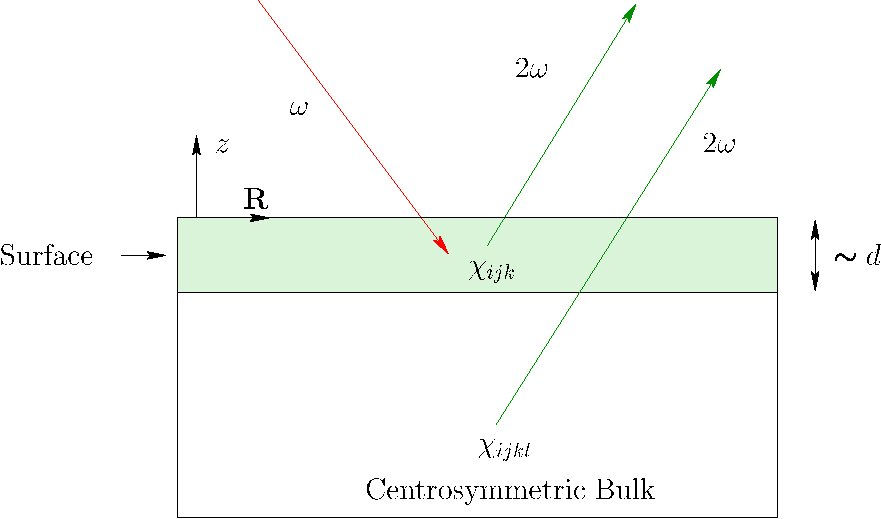
\includegraphics[scale=0.6]{figures/images/system.pdf}
\caption{(Color Online) Sketch of the semi-infinite system with a 
centrosymmetric bulk. The surface region is of width $\sim d$. 
The incoming photon of frequency $\go$ is represented by
a downward red arrow, whereas both the surface and bulk created second
harmonic photons of frequency $2\go$ are represented by upward
green arrows. The red color suggests an incoming infrared photon with
a green second harmonic photon. The dipolar ($\chi_{\rma\rmb\rmc}$), and 
quadrupolar ($\chi_{\rma\rmb\rmc\rml}$) susceptibility tensors are shown 
in the regions where they are different from zero. The axis has $z$
perpendicular to the surface and $\mbf{R}$ parallel to it.\label{fsystem}}
\end{figure}

If we move to the surface of the semi-infinite system our assumption 
of centrosymmetry breaks down, and there is no restriction in 
$\chi_{\rma\rmb\rmc}$. We conclude that the leading term
of the polarization in a surface region is given by
\begin{align}\label{sshgp1}
\int dz 
P_{\rma}(\mbf{R},z)
\approx dP_{\rma}
\equiv
P_{\rma}^S
\equiv
\chi^S_{\rma\rmb\rmc}E_{\rmb}E_{\rmc},
\end{align}
where
% $\mbf{R}$ is a vector parallel to the surface which is
% perpendicular to $z$, $\cals$ is the surface area of the unit
% cell that characterizes the surface of the system, and 
$d$ is the
surface region from which the dipolar signal of $\bfP$ is
different from zero (see Fig.~\ref{fsystem}), and
$\mbf{P}^S\equiv d\mbf{P}$
 is the surface SH polarization. Then, from Eq.~\eqref{mshg} we obtain that
\begin{align}\label{sshgp2}
\chi_{\rma\rmb\rmc}^S=d\chi_{\rma\rmb\rmc}
\end{align}
is the
SH surface susceptibility. 
On the other hand, 
\begin{equation}\label{sshgp3}
P^b_{\rma}(\mbf{r})=\chi_{\rma\rmb\rmc\rml}E_{\rmb}(\mbf{r})\nabla_{\rmc}
E_{\rml}(\mbf{r}),  
\end{equation}
gives the bulk polarization. We immediately recognize that the surface
polarization is of dipolar order while the bulk polarization is of
quadrupolar order. The surface, $\chi^S_{\rma\rmb\rmc}$, and bulk, 
$\chi_{\rma\rmb\rmc\rml}$, susceptibility tensor ranks are three and 
four, respectively. We will only concentrate on surface SHG in this article 
even though bulk generated SH is also a very important optical phenomenon. 
Also, we leave out of this article other interesting surface SH phenomena like, electric field
induced second harmonic (EFISH), which would be represented by a
surface susceptibility  tensor of quadrupolar origin.
In centrosymmetric systems for which the quadrupolar bulk
response is much smaller than the dipolar surface response, SH is
readily used as a very useful and powerful 
optical surface probe.\cite{downer_optical_2001}

In the following sections we present the theoretical approach to
derive
the expressions for the 
surface susceptibility tensor $\chi^S_{\rma\rmb\rmc}$.

\section{Length Gauge}\label{longi}

We follow the article by Aversa and Sipe\cite{aversaPRB95} to calculate 
the optical properties of a given system within the longitudinal gauge. 
More recent derivations
can also be found in Refs. \cite{sipe_second-order_2000,lambrechtPSSB00}.  
Assuming the long-wavelength approximation which implies 
a position independent electric field, 
$\bfE(t)$,  
the Hamiltonian in the length gauge approximation is given by
\begin{equation}\label{ache}
\hat{H}=\hat{H}^\gs_0-e \hat\bfr \cdot \bfE,
\end{equation}
with
\begin{align}\label{ache.1}
\hat H^\gs_0=\hat H^\lda_0
 + \cals(\bfr,\bfp)
,
\end{align} 
as the unperturbed Hamiltonian.
The LDA Hamiltonian can be expressed as follows,
\begin{align}\label{ache.2}
\hat H^\lda_0&=\frac{\hat p^2}{2m_e}  + \hat V^\ps
\nonumber\\
\hat V^\ps
&=\hat V^l(\hat\bfr) + \hat V^\nl
,
\end{align}  
where $\hat V^l(\hat\bfr)$ and $\hat V^\nl$ are the local and
the non-local parts of the  
crystal 
pseudopotential $\hat V^\ps$. For the latter, we have that
\begin{align}\label{ache.3n}
 V^\nl(\bfr,\bfr')
\equiv \bra{\bfr}\hat V^\nl\ket{\bfr'}\neq 0 \quad\mathrm{for}\quad\bfr\neq\bfr'
,
\end{align}
where $V^\nl(\bfr,\bfr')$ is a function of $\bfr$ and $\bfr'$
representing the non-local contribution of the pseudopotential.
The Schr\"odinger equation reads
\begin{align}\label{ache.4} 
\left(
\frac{-\hbar^2}{2m_e}\nabla^2
 + \hat V^l(\bfr)\right)\psi_{n\bfk}(\bfr)
 + \int d\bfr'\hat V^\nl(\bfr,\bfr')\psi_{n\bfk}(\bfr')
=E_i\psi_{n\bfk}(\bfr)
,
\end{align} 
where
%$\psi_{n\bfk}(\bfr)=\braket{\bfr}{n\bfk}=\sqrt{\gO/8\pi^3}e^{i\bfk\cdot\bfr}u_{n\bfk}(\bfr)$,
$\psi_{n\bfk}(\bfr)=\braket{\bfr}{n\bfk}=e^{i\bfk\cdot\bfr}u_{n\bfk}(\bfr)$,
are the real space representations of the Bloch states $\ket{n\bfk}$ labelled
by the band index $n$ and the crystal momentum $\bfk$, and $u_{n\bfk}(\bfr)$
is cell periodic. $m_e$ is the bare mass of the electron and $\gO$ is the 
unit cell volume. The nonlocal scissors operator is given by 
\begin{equation}\label{chon.0}
\cals(\bfr,\bfp)=\hbar\gS\sum_n\int d^3k'(1-f_n(\bfk)) \ket{n\bfk'}\bra{n\bfk'}
,
\end{equation}
where $f_n(\bfk)$ is the occupation number, that for $T=0$ K, is
independent of $\bfk$, and is one for filled bands and zero for
unoccupied bands. For semiconductors the filled bands correspond to
valence
bands  ($n=v$) and the unoccupied bands to conduction bands
 ($n=c$). 
We have that
\begin{align}\label{chon.1}  
H^\lda_0\ket{n\bfk}&=\hbar\go^\lda_n(\bfk)\ket{n\bfk}
\nonumber\\
H^\gs_0\ket{n\bfk}&=\hbar\go^\gs_n(\bfk)\ket{n\bfk}
,
\end{align} 
where 
\begin{align}\label{chon.78}
\hbar\go^\gs_n(\bfk)=\hbar\go^\lda_n(\bfk)+\hbar\gS(1-f_n)
,
\end{align}
is the
 scissored
energy. Here, 
$\hbar\gS$ is the value by which the conduction bands are rigidly
($\bfk$-independent)
 shifted
upwards in energy, also known as the scissors shift. $\gS$ could be taken to be
$\bfk$ dependent, but for most calculations (like the ones presented
here), a rigid shift is sufficient. We can take 
$\hbar\gS=E_g-E_g^\lda$ where $E_g$ could be the experimental band gap 
or GW band gap taken at the $\Gamma$ point, i.e. $\bfk=0$.
We used the fact that 
$\ket{n\bfk}^\lda\approx\ket{n\bfk}^\gs$, thus negating the need to label
the Bloch states with the LDA or $\gs$ superscripts. 
The matrix elements of $\bfr$ are split between the {\it intraband} 
($\bfr_i$) and {\it interband} ($\bfr_e$) parts , where 
$\bfr=\bfr_i+\bfr_e$ and\cite{adamsJCP53,blountSSP62,aversaPRB95}
\begin{align}\label{rnminn}
\bra{n\bfk}\hat\bfr_i\ket{m\bfk'} &= \gd_{nm}\left[\gd(\bfk-\bfk')\bfgxi_{nn}(\bfk)
+i\nabla_\bfk\gd(\bfk-\bfk')\right], \\
\bra{n\bfk}\hat\bfr_e\ket{m\bfk'} &=
(1-\gd_{nm})\gd(\bfk-\bfk')\bfgxi_{nm}(\bfk)
,
\label{rnmenn}
\end{align}
and
\begin{equation}\label{zetann}
\bfgxi_{nm}(\bfk) \equiv i\frac{(2\pi)^3}{\gO}\int_{\gO} d\bfr\, u^*_{n\bfk}(\bfr)\nabla_{\bfk}u_{m\bfk}(\bfr).
\end{equation}
The interband part $\bfr_e$ can
be obtained as follows. 
We start by introducing the 
velocity operator
\begin{align}\label{vop}
\hat\bfv^\gs&=
\frac{1}{i\hbar}[\hat\bfr,\hat{H}^\gs_0]
,
\end{align}
and calculating its matrix elements
\begin{equation}\label{conhrnm}
i\hbar\bra{n\bfk}
\bfv^\gs
\ket{m\bfk}
=
\bra{n\bfk}
[\hat\bfr,\hat{H}^\gs_0]
\ket{m\bfk}
=\bra{n\bfk}\hat\bfr\hat{H}^\gs_0-\hat{H}^\gs_0\hat\bfr\ket{m\bfk}
=(\hbar\go^\gs_m(\bfk)-\hbar\go^\gs_n(\bfk))\bra{n\bfk}\hat\bfr\ket{m\bfk}
,
\end{equation}
thus defining $\go^\gs_{nm}(\bfk)=\go^\gs_n(\bfk)-\go^\gs_m(\bfk)$ we get
\begin{align}\label{pmnrmn}
\bfr_{nm}(\bfk)
&=
\frac{\bfv^\gs_{nm}(\bfk)}{i\go^\gs_{nm}(\bfk)}
\quad\quad n\notin D_m
,
\end{align} 
which can be identified as 
$\bfr_{nm}=(1-\gd_{nm})\bfgxi_{nm}\to \bfr_{e,nm}$.
Here, $D_m$ are all the possible degenerate $m$-states.
When $\bfr_i$ appears in
commutators we use\cite{aversaPRB95} 
\begin{equation}\label{conmri3n}
\bra{n\bfk}[\hat\bfr_i,\hat\calo]\ket{m\bfk'}
=i\gd(\bfk-\bfk')(\calo_{nm})_{;\bfk}
,
\end{equation}  
with
\begin{equation}\label{gendevnn}
(\calo_{nm})_{;\bfk}=
\nabla_\bfk
\calo_{n m}(\bfk)
- 
i
\calo_{nm}(\bfk)
\left(
\bfgxi_{nn}(\bfk)
-
\bfgxi_{mm}(\bfk)
\right)
,
\end{equation} 
where ``$;\bfk$'' denotes the generalized derivative (see Appendix \ref{reri}). 

As can be seen from Eq.~\eqref{ache.1} and \eqref{ache.2},
both $\hat S$ and $\hat V^\nl$ are nonlocal potentials. Their contribution 
in the calculation of the optical response has to be taken in order to
get reliable results.\cite{ismailPRL01}
We proceed as follows; from Eqs.~\eqref{vop}, \eqref{ache.1} and
\eqref{ache.2}
 we find
\begin{align}\label{vop2}
\hat\bfv^\gs&=
\frac{\hat\bfp}{m_e}
+
\frac{1}{i\hbar}[\hat\bfr,\hat V^\nl(\bfr,\bfr')]
+
\frac{1}{i\hbar}[\hat\bfr,\hat\cals(\bfr,\bfp)]
\nonumber\\
&\equiv
\hat\bfv
+
\hat\bfv^\nl
+\hat\bfv^\cals
=
\hat\bfv^\lda
+\hat\bfv^\cals
,
\end{align}
where we have defined
\begin{align}\label{conhr}
\hat\bfv
&=\frac{\hat\bfp}{m_e}
\nonumber\\
\hat\bfv^\nl
&=
\frac{1}{i\hbar}[\hat\bfr,\hat V^\nl]
\nonumber\\
\hat\bfv^\cals
&=
\frac{1}{i\hbar}[\hat\bfr,\hat S(\bfr,\bfp)]
\nonumber\\
\hat\bfv^\lda
&=
\hat\bfv
+\hat\bfv^\nl
\end{align}  
with $\hat\bfp=-i\hbar\bfgnabla$ the momentum operator.
Using Eq.~\eqref{chon.0}, we obtain that the
matrix elements of $\hat\bfv^\cals$ are given by
\begin{equation}\label{chon.2} 
\bfv^\cals_{nm}=i\gS f_{mn}\bfr_{nm},
%=\frac{\gS f_{mn}}{\go^\lda_{nm}}\bfv^\lda_{nm}
\end{equation}
with $f_{nm}=f_n-f_m$,
where we see that $\bfv^\cals_{nn}=0$, then
\begin{align}\label{chon.8}
\bfv^\gs_{nm}
&=
\bfv^\lda_{nm}+i\gS f_{mn}\bfr_{nm}
\nonumber\\
&=
\bfv^\lda_{nm}+i\gS f_{mn}\frac{\bfv^\gs_{nm}(\bfk)}{i\go^\gs_{nm}(\bfk)}
\nonumber\\
\bfv^\gs_{nm}
\frac{\go^\gs_{nm}-\gS f_{mn}}{\go^\gs_{nm}}
&=
\bfv^\lda_{nm}
\nonumber\\
\bfv^\gs_{nm}
\frac{\go^\lda_{nm}}{\go^\gs_{nm}}
&=
\bfv^\lda_{nm}
\nonumber\\
\frac{\bfv^\gs_{nm}}{\go^\gs_{nm}}
&=
\frac{\bfv^\lda_{nm}}{\go^\lda_{nm}}
,
\end{align}
since
$\go^\gs_{nm}-\gS f_{mn}=\go^\lda_{nm}$. Therefore, 
\begin{align}\label{chon.9}
\bfv^\gs_{nm}(\bfk)
&=
\frac{\go^\gs_{nm}}{\go^\lda_{nm}}\bfv^\lda_{nm}(\bfk)
=\left(1+\frac{\gS}{\go_c(\bfk)-\go_v(\bfk)}\right)\bfv^\lda_{nm}(\bfk)
\quad\quad n\notin D_m
\nonumber\\
\bfv^\gs_{nn}(\bfk)
&=
\bfv^\lda_{nn}(\bfk)
,
\end{align} 
and Eq.~\eqref{pmnrmn} gives
\begin{align}\label{chon.10}
\bfr_{nm}(\bfk)
=
\frac{\bfv^\gs_{nm}(\bfk)}{i\go^\gs_{nm}(\bfk)}
=
\frac{\bfv^\lda_{nm}(\bfk)}{i\go^\lda_{nm}(\bfk)}
\quad\quad n\notin D_m
.
\end{align}
The matrix elements
of $\bfr_e$ are the same whether we use the LDA or the scissored
Hamiltonian and there is no need to label them with either LDA
or S superscripts. Thus,
we can write
\begin{equation}\label{chon.98}
\bfr_{e,nm}\to
\bfr_{nm}(\bfk)=\frac{\bfv^\lda_{nm}(\bfk)}{i\go^\lda_{nm}(\bfk)}
\quad\quad n\notin D_m
,
\end{equation}   
which gives the interband matrix elements of the position operator
in terms of the matrix elements of $\hat\bfv^\lda$. 
These matrix elements include the matrix elements of
$\bfv^\nl_{nm}(\bfk)$ which can be readily calculated\cite{francesco} for 
fully separable nonlocal pseudopotentials in the 
Kleinman-Bylander 
form.\cite{mottaCMS10,kleinman_efficacious_1982,adolphPRB96}
In Appendix \ref{appvnl} we outline how this  
can be accomplished. 

\section{Time-dependent Perturbation Theory}\label{tdpt}

In the independent particle approximation, we use the electron density
operator $\hat\gr$ to obtain the expectation value of any observable
$\calo$ as
\begin{equation}\label{traza}
\calo=\mathrm{Tr}(\hat\calo\hat\rho)=\mathrm{Tr}(\hat\rho\hat\calo),
\end{equation}
where $\mathrm{Tr}$ is the trace and is invariant under cyclic permutations.
The dynamic equation of motion for $\gr$ is given by
\begin{equation}\label{eqrho}
i\hbar \frac{d\hat\gr}{dt}=[\hat{H},\hat\gr]
,
\end{equation}
where it is more convenient to work in the interaction picture. We transform 
all operators according to 
\begin{equation}\label{ip}
\hat{\calo}_I=\hat{U}\hat{\calo}\hat{U}^\dagger,
\end{equation}
where
\begin{equation}\label{ou}
\hat{U}=e^{i\hat{H}_0t/\hbar},
\end{equation}
is the unitary operator that shifts us to the interaction picture.
Note that $\hat\calo_I$ depends on time even if $\hat\calo$ does not.
Then, we transform Eq.~\eqref{eqrho} into
\begin{equation}\label{intrho}
i\hbar\frac{d\hat\gr_I(t)}{dt}=[-e\hat\bfr_I(t)\cdot\bfE(t),\hat\gr_I(t)],
\end{equation}
that leads to
\begin{equation}\label{intrho2}
\hat\gr_I(t)=\hat\gr_I(t=-\infty)
+
\frac{ie}{\hbar}\int_{-\infty}^t dt'[\hat\bfr_I(t')\cdot\bfE(t'),\hat\gr_I(t')].
\end{equation}
We assume that the interaction is switched-on adiabatically and
choose a time-periodic perturbing field, to write
\begin{equation}\label{efield}
\bfE(t)=\bfE e^{-i\go t}e^{\eta t}=\bfE e^{-i\got t}
,
\end{equation}
with
\begin{equation}\label{got}
\got=\go+i\eta
,
\end{equation} 
where $\eta > 0$ assures
that at $t=-\infty$ the interaction is zero and has its full strength $\bfE$ 
at $t=0$. After computing the required time integrals one takes
$\eta\to 0$. 
Also, $\hat\gr_I(t=-\infty)$ should be time independent and thus 
$[\hat{H},\hat\rho]_{t=-\infty}=0$, This implies that 
$\hat\gr_I(t=-\infty)=\hat\rho(t=-\infty)\equiv\hat\rho_0$,
where $\hat\rho_0$ is
the density matrix of the unperturbed ground state,
such that
\begin{equation}\label{nrhon}
\bra{n\bfk}\hat\gr_0\ket{m\bfk'}=f_n(\hbar\go^\gs_n(\bfk))\gd_{nm}\gd(\bfk-\bfk')
,
\end{equation}
with $f_n(\hbar\go^\gs_n(\bfk))=f_{n\bfk}$ as the Fermi-Dirac distribution function.

We solve Eq.~\eqref{intrho2} using the standard iterative
solution, for which we write
\begin{equation}\label{rhop}
\hat\rho_I=\hat\rho_I^{(0)}+\hat\rho_I^{(1)}+\hat\rho_I^{(2)}+\cdots
,
\end{equation}
where $\hat\rho_I^{(N)}$ is the density operator to order $N$ in $\bfE(t)$.
Then, Eq.~\eqref{intrho2} reads
\begin{equation}\label{intrho3}
\hat\rho_I^{(0)}+\hat\rho_I^{(1)}+\hat\rho_I^{(2)}+\cdots
=\hat\gr_0
+
\frac{ie}{\hbar}\int_{-\infty}^t dt'[\hat\bfr_I(t')\cdot\bfE(t'),
\hat\rho_I^{(0)}+\hat\rho_I^{(1)}+\hat\rho_I^{(2)}+\cdots
]
,
\end{equation}
where, by equating equal orders in the perturbation, we find
\begin{equation}\label{rho0}
\hat\gr_I^{(0)}\equiv\hat\gr_0
,
\end{equation}
and
\begin{equation}\label{rhoN}
\hat\gr_I^{(N)}(t)=
\frac{ie}{\hbar}
\int_{-\infty}^t dt'[\hat\bfr_I(t')\cdot\bfE(t'),\hat\gr^{(N-1)}_I(t')].
\end{equation}
It is simple to show that matrix elements of Eq. (\ref{rhoN}) satisfy
$\bra{n\bfk}\gr_I^{(N+1)}(t)\ket{m\bfk'}=\gr^{(N+1)}_{I,nm}(\bfk)\gd(\bfk-\bfk')$,
with
\begin{equation}\label{rtilde}
\gr^{(N+1)}_{I,nm}(\bfk;t)
=\frac{ie}{\hbar}\int_{-\infty}^t dt'
\bra{n\bfk}
[\hat\bfr_I(t'),\hat\gr^{(N)}_I(t')]
\ket{m\bfk}
\cdot\bfE(t')
.
\end{equation}

We now work out the commutator of Eq.~\eqref{rtilde}. Then,
\begin{align}\label{conmu1}
\bra{n\bfk}
[\hat\bfr_I(t),\hat\gr^{(N)}_I(t)]
\ket{m\bfk}
&=
\bra{n\bfk}
[\hat{U}\hat\bfr\hat{U}^\dagger,\hat{U}\hat\gr^{(N)}(t)\hat{U}^\dagger]
\ket{m\bfk}
\nonumber \\
&=
\bra{n\bfk}
\hat{U}[\hat\bfr,\hat\gr^{(N)}(t)]\hat{U}^\dagger
\ket{m\bfk}
\\
&=
e^{i\go^\gs_{nm\bfk}t}
\left(
\bra{n\bfk}
[\hat\bfr_e,\hat\gr^{(N)}(t)]
+
[\hat\bfr_i,\hat\gr^{(N)}(t)]
\ket{m\bfk}
\right)
\nonumber
.
\end{align}
% where the time dependence of operator's interaction picture is
% explicitly shown by the exponential factor, and the implicit
% dependence of $\hat\rho^{(N)}$ inherited from Eq.~\eqref{eqrho} is
% shown by its $t$ argument.
We calculate the interband term first, so using Eq.~\eqref{chon.98} we obtain
\begin{align}\label{conmu2}
\bra{n\bfk}
[\hat\bfr_e,\hat\gr^{(N)}(t)]
\ket{m\bfk}
&=
\sum_{\ell}
\left(
\bra{n\bfk}
\hat\bfr_e
\ket{\ell\bfk}
\bra{\ell\bfk}
\hat\gr^{(N)}(t)
\ket{m\bfk}
\right.
\nonumber \\
&
\left.
-
\bra{n\bfk}
\hat\gr^{(N)}(t)
\ket{\ell\bfk}
\bra{\ell\bfk}
\hat\bfr_e
\ket{m\bfk}
\right)
\nonumber \\
&=
\sum_{\ell\ne n,m}
\left(
\bfr_{n\ell}(\bfk)
\gr^{(N)}_{\ell m}(\bfk;t)
-
\gr^{(N)}_{n\ell}(\bfk;t)
\bfr_{\ell m}(\bfk)
\right)
\nonumber\\
&\equiv
\bfR^{(N)}_e(\bfk;t)
,
\end{align}

and from Eq.~\eqref{conmri3n},
\begin{equation}\label{conmri4}
\bra{n\bfk}[\hat\bfr_i,\hat\rho^{(N)}(t)]\ket{m\bfk'}
=i \gd(\bfk-\bfk') (\rho^{(N)}_{nm}(t))_{;\bfk}
\equiv \gd(\bfk-\bfk')\bfR_i^{(N)}(\bfk;t)
.
\end{equation}
Then Eq.~\eqref{rtilde} becomes
\begin{equation}\label{rtilde2}
\gr^{(N+1)}_{I,nm}(\bfk;t)
=\frac{ie}{\hbar}\int_{-\infty}^t dt'
e^{i(\go^\gs_{nm\bfk}-\got)t'}
\left[R_e^{\rmb(N)}(\bfk;t')+R_i^{\rmb(N)}(\bfk;t')\right]E^{\rmb}
,
\end{equation}
where the roman superindices
$\rma,\rmb,\rmc$ denote Cartesian components that are summed over if repeated.
Starting from the linear response and proceeding from Eq.~\eqref{nrhon} and ~\eqref{conmu2},
\begin{align}\label{R0e}
R_e^{\rmb(0)}(\bfk;t)
&=
\sum_{\ell}
\left(
r^{\rmb}_{n\ell}(\bfk)
\gr^{(0)}_{\ell m}(\bfk)
-
\gr^{(0)}_{n\ell}(\bfk)
r^{\rmb}_{\ell m}(\bfk)
\right)
\nonumber \\
&=
\sum_{\ell}
\left(
r^{\rmb}_{n\ell}(\bfk)
\gd_{\ell m}f_m(\hbar\go^\gs_m(\bfk))
-
\gd_{n\ell}f_n(\hbar\go^\gs_n(\bfk))
r^{\rmb}_{\ell m}(\bfk)
\right)
\nonumber \\
&=
f_{mn\bfk}
r^{\rmb}_{nm}(\bfk)
,
\end{align}
where $f_{mn\bfk}=f_{m\bfk}-f_{n\bfk}$.
From now on,
it should be clear that the matrix elements of $\bfr_{nm}$ imply
$n\notin D_m$.
We also have from Eq.~\eqref{conmri4} and Eq.~\eqref{gendevnn} that
\begin{equation}\label{R0i}
R_i^{\rmb(0)}(\bfk)=i(\rho^{(0)}_{nm})_{;k^{\rmb}}=i\gd_{nm}(f_{n\bfk})_{;k^{\rmb}}=i\gd_{nm}\nabla_{k^{\rmb}} f_{n\bfk}
.
\end{equation}
For a semiconductor at $T=0$, $f_{n\bfk}$ is one if the state
$\ket{n\bfk}$ is a valence state and zero if it is a conduction state; 
thus $\nabla_\bfk f_{n\bfk}=0$ and $\bfR_i^{(0)}=0$ and
the linear response has no contribution from
intraband transitions.
 Then,
\begin{align}\label{rtilde2n}
\gr^{(1)}_{I,nm}(\bfk;t)
&=\frac{ie}{\hbar}
f_{mn\bfk}
r^{\rmb}_{nm}(\bfk)E^{\rmb}
\int_{-\infty}^t dt'
e^{i(\go^\gs_{nm\bfk}-\got)t'}
\nonumber \\
&=\frac{e}{\hbar}
f_{mn\bfk}
r^{\rmb}_{nm}(\bfk)E^{\rmb}
\frac{e^{i(\go^\gs_{nm\bfk}-\got)t}}
{\go^\gs_{nm\bfk}-\got}
\nonumber \\
&=
e^{i\go^\gs_{nm\bfk}t}
B^{\rmb}_{mn}(\bfk)E^{\rmb}(t)
\nonumber \\
&=
e^{i\go^\gs_{nm\bfk}t}
\rho^{(1)}_{nm}(\bfk;t)
,
\end{align}
with
\begin{equation}\label{rho1} 
B^{\rmb}_{nm}(\bfk,\go)=
\frac{e}{\hbar}\frac{f_{mn\bfk}r^{\rmb}_{nm}(\bfk)}{\go^\gs_{nm\bfk}-\got}
,
\end{equation} 
and
\begin{equation}\label{rhonoi1}
\rho^{(1)}_{nm}(\bfk;t)=B^{\rmb}_{mn}(\bfk,\go)E^{\rmb}(\go)e^{-i\got t}
.
\end{equation}

Now, we calculate the second-order response. Then, from Eq.~\eqref{conmu2}
\begin{align}\label{R1e}
R_e^{\rmb(1)}(\bfk;t)
&=
\sum_{\ell}
\left(
r^{\rmb}_{n\ell}(\bfk)
\gr^{(1)}_{\ell m}(\bfk;t)
-
\gr^{(1)}_{n\ell}(\bfk;t)
r^{\rmb}_{\ell m}(\bfk)
\right)
\nonumber \\
&=
\sum_{\ell}
\left(
r^{\rmb}_{n\ell}(\bfk)
B^{\rmc}_{\ell m}(\bfk,\go)
-
B^{\rmc}_{n\ell}(\bfk,\go)
r^{\rmb}_{\ell m}(\bfk)
\right)E^{\rmc}(t)
,
\end{align}
and from Eq.~\eqref{conmri4}
\begin{equation}\label{R1i}
R_i^{\rmb(1)}(\bfk;t)=
i(\rho^{(1)}_{nm}(t))_{;k^{\rmb}}=
iE^{\rmc}(t)(B^{\rmc}_{nm}(\bfk,\go))_{;k^{\rmb}}
.
\end{equation}

Using Eqs.~\eqref{R1e} and ~\eqref{R1i} in Eq. (\ref{rtilde2}),
we obtain
\begin{align}\label{rtilde33}
\gr^{(2)}_{I,nm}(\bfk;t)
&=
\frac{ie}{\hbar}
\bigg[
\sum_{\ell}
\Big(
r^{\rmb}_{n\ell}(\bfk)
B^{\rmc}_{\ell m}(\bfk,\go)
-
B^{\rmc}_{n\ell}(\bfk,\go)
r^{\rmb}_{\ell m}(\bfk)
\Big)
\nonumber \\
&+
i
(B^{\rmc}_{nm}(\bfk,\go))_{;k^{\rmb}}
\bigg]
E^{\rmb}_{\go}E_{\go}^{\rmc}
\int_{-\infty}^t dt'
e^{i(\go^\gs_{nm\bfk}-2\got)t'}
\nonumber \\
&=
\frac{e}{\hbar}
\bigg[
\sum_{\ell}
\Big(
r^{\rmb}_{n\ell}(\bfk)
B^{\rmc}_{\ell m}(\bfk,\go)
-
B^{\rmc}_{n\ell}(\bfk,\go)
r^{\rmb}_{\ell m}(\bfk)
\Big)
\nonumber \\
&+
i
(B^{\rmc}_{nm}(\bfk,\go))_{;k^{\rmb}}
\bigg]
E^{\rmb}_{\go}E_{\go}^{\rmc}
\frac{e^{i(\go^\gs_{nm\bfk}-2\got)t}}
{\go^\gs_{nm\bfk}-2\got}
\nonumber \\
&=
e^{i\go^\gs_{nm\bfk}t}
\rho_{nm}^{(2)}(\bfk;t)
.
\end{align}
Now, we write
$\rho_{nm}^{(2)}(\bfk;t)=\rho_{nm}^{(2)}(\bfk;2\go)e^{-i2\got t}$,
with
\begin{align}\label{rho2}
\gr_{nm}^{(2)}(\bfk;2\go)&=\frac{e}{i\hbar}\frac{1}{\go^\gs_{nm\bfk}-2\got}
\bigg[-(B_{nm}^{\rmc}(\bfk,\go)_{;k^{\rmb}}
\nonumber \\
&
+i\sum_\ell\Big(r_{n\ell}^{\rmb}B_{\ell m}^{\rmc}(\bfk,\go) - B_{n\ell}^{\rmc}(\bfk,\go)
  r_{\ell m}^{\rmb}\Big)
\bigg] 
E^{\rmb}(\go)E^{\rmc}(\go)
\end{align} 
where 
$B_{\ell m}^{\rma}(\bfk,\go)$ are given by Eq.~\eqref{rho1}. 
We remark that $\bfr_{nm}(\bfk)$  are
the same whether calculated with the LDA or the scissored Hamiltonian. 
We chose the former in this article.

\section{Layered Current Density}\label{cd}

In this section, we derive the expressions for the microscopic current
density of a given layer in the unit cell of the system.
The approach we use to study the surface of a semi-infinite
semiconductor crystal is as follows. Instead of using a
semi-infinite system, we replace it by a slab (see Fig.~\ref{fslab}).
The slab consists of a front and back surface, and in between these
two surfaces is the bulk of the system. 
In general the surface of a crystal reconstructs or relaxes as the atoms
move to find equilibrium positions. This is due to the fact that
the otherwise
balanced forces are disrupted when the surface atoms do not find their 
partner atoms that are now absent at the surface of the slab. 

To take the reconstruction or relaxation into account, we take ``surface'' to mean
the true surface of the first layer of atoms, and
some of the atomic sub-layers adjacent to it.
Since the front and the back
surfaces of the slab are usually identical the total slab is
centrosymmetric. This implies that 
$\chi^{\mathrm{slab}}_{\rma\rmb\rmc}=0$, and thus we must
find a way to bypass this characteristic of a centrosymmetric slab 
in order to have a finite $\chi^s_{\rma\rmb\rmc}$ representative of the
surface. Even if the front and back surfaces of the slab 
are different, breaking the centrosymmetry and therefore giving an
overall $\chi^{\mathrm{slab}}_{\rma\rmb\rmc}\ne 0$, we still
need a procedure to extract the front surface $\chi^f_{\rma\rmb\rmc}$
and the back surface $\chi^b_{\rma\rmb\rmc}$ from the non-linear
susceptibility 
$\chi^{\mathrm{slab}}_{\rma\rmb\rmc}=\chi^f_{\rma\rmb\rmc}-\chi^b_{\rma\rmb\rmc}$
 of the entire slab.

A convenient way to accomplish the separation of the SH signal of
either surface is to introduce a ``cut function'', $\calc(z)$, which is 
usually taken to be unity over one half of the slab and zero over 
the other half.\cite{reining_microscopic_1994}
 In this case $\calc(z)$ will give the contribution of the 
side of the slab for which $\calc(z)=1$. We can generalize this 
simple choice for $\calc(z)$ by a top-hat cut function
$\calc^\ell(z)$ that selects a given layer,
\begin{equation}
\label{sz}
\calc^\ell(z)=\Theta(z-z_\ell+\Delta_\ell^{\rmb})
            \Theta(z_\ell-z+\Delta_\ell^f),
\end{equation}
where $\Theta$ is the Heaviside function. Here, $\Delta_\ell^{f/b}$
is the distance that the $\ell$-th layer extends towards the front
$(f)$ or back $(b)$ from its $z_\ell$ position. 
$\Delta_\ell^f+\Delta_\ell^b$ is the thickness of layer $\ell$ 
(see Fig.~\ref{fslab}).
\begin{figure}[b]
\centering
%\includegraphics[height=5cm,width=7cm]{slab}
\includegraphics[scale=.7]{figures/images/slab.pdf}
\caption{A sketch of a slab where the circles represent atoms.\label{fslab}}
\end{figure}

Now, we show how this ``cut function'' $\calc^\ell(z)$ is introduced in
the calculation of $\chi_{\rma\rmb\rmc}$. 
The microscopic current density is given by
\begin{equation}\label{jmic}
\bfj(\bfr,t)=\mathrm{Tr}(\hat\bfj(\bfr)\hat\rho(t)),
\end{equation}
where the operator for the electron's current is
\begin{equation}\label{hatjmic}
\hat\bfj(\bfr)=\frac{e}{2}\left(\hat\bfv^\gs\ket{\bfr}\bra{\bfr}
+\ket{\bfr}\bra{\bfr}\hat\bfv^\gs\right), 
\end{equation}
where $\hat{\mbf{v}}^\gs$ is the electron's velocity operator to be dealt
with below. We define
$\hat\mu\equiv\ket{\bfr}\bra{\bfr}$ and use the cyclic invariance of
the trace to write
\begin{align}\label{jmic2}
\mathrm{Tr}(\hat\bfj(\bfr)\hat\rho(t)&=\mathrm{Tr}(\hat\rho(t)\hat\bfj(\bfr))=
\frac{e}{2}
\left(
\mathrm{Tr}(\hat\rho\hat\bfv^\gs\hat\mu)
+
\mathrm{Tr}(\hat\rho\hat\mu\hat\bfv^\gs)
\right)
\nonumber\\
&=
\frac{e}{2}
\sum_{n\bfk}
\left(
\bra{n\bfk}\hat\rho\hat\bfv^\gs\hat\mu\ket{n\bfk}
+
\bra{n\bfk}\hat\rho\hat\mu\hat\bfv^\gs\ket{n\bfk}
\right)
\nonumber\\
&=
\frac{e}{2}
\sum_{nm\bfk}
\bra{n\bfk}\hat\rho\ket{m\bfk}
\left(
\bra{m\bfk}\hat\bfv^\gs\ket{\bfr}\braket{\bfr}{n\bfk}
+
\braket{m\bfk}{\bfr}\bra{\bfr}\hat\bfv^\gs\ket{n\bfk}
\right)
\nonumber\\
\bfj(\bfr,t)&=
\sum_{nm\bfk}
\rho_{nm}(\bfk;t)\bfj_{mn}(\bfk;\bfr),
\end{align}
where
\begin{equation}\label{jmic3}
\bfj_{mn}(\bfk;\bfr)=
\frac{e}{2}
\left(
\bra{m\bfk}\hat\bfv^\gs\ket{\bfr}\braket{\bfr}{n\bfk}
+
\braket{m\bfk}{\bfr}\bra{\bfr}\hat\bfv^\gs\ket{n\bfk}
\right),
\end{equation}
are the matrix elements of the microscopic current operator,
and we have used the fact that the matrix elements between states $\ket{n\bfk}$
are diagonal in $\bfk$, i.e. proportional to $\gd(\bfk-\bfk')$.

Integrating the microscopic current $\mbf{j}(\mbf{r},t)$ over
the entire slab gives the averaged microscopic current density. 
If we want the contribution from only one region of the unit cell 
towards the total current, we can integrate $\mathbf{j}({\mathbf r},t)$ 
over the desired region. The contribution to the current density from the
$\ell$-th layer of the slab is given by
\begin{equation}\label{jsz}
\frac{1}{\Omega}\int d^3r\, \calc^\ell(z)\, \mathbf{j}(\mathbf{r},t)
 \equiv \mathbf{J}^{\ell}(t),
\end{equation}
where $\mathbf{J}^{\ell}(t)$ is the microscopic current in the
$\ell$-th layer.
Therefore we define
\begin{equation}\label{vcal}
e{\boldsymbol{\mathcal{V}}}^{\gs,\ell}_{mn}(\mathbf{k})
\equiv
%\frac{1}{\Omega}
\int d^3r\, \calc^\ell(z)\,\bfj_{mn}({\bfk};\bfr),
\end{equation}
to write
\begin{equation}\label{jmac}
J_a^{(N,\ell)}(t)=\frac{e}{\gO}
\sum_{mn\bfk}
\mathcal{V}^{\gs,a,\ell}_{mn}(\mathbf{k})
\rho^{(N)}_{nm}(\bfk;t),
\end{equation}
as the induced microscopic current of the $\ell$-th layer, to order $N$ 
in the external perturbation. The matrix elements of the 
density operator for $N=1,2$ are given by Eqs.~\eqref{rho1} and
\eqref{rho2} respectively. 
The Fourier component of microscopic current of Eq.~\eqref{jmac} is given by
\begin{equation}\label{jmac2}
J_{\rma}^{(N,\ell)}(\go_3)=\frac{e}{\gO}
\sum_{mn\bfk}
\calv^{\gs,\rma,\ell}_{mn}(\mathbf{k})
\rho^{(N)}_{nm}(\bfk;\go_3)
.
\end{equation}
We proceed to give an explicit expression of
$\calbv^{\gs,\ell}_{mn}(\mathbf{k})$.
From
Eqs.~\eqref{vcal} and \eqref{jmic3} we obtain
\begin{equation}\label{intj}
{\boldsymbol{\mathcal{V}}}^{\gs,\ell}_{mn}({\mathbf k})=
\frac{1}{2}
\int \mathrm{d}^3 r\,
 \calc^\ell(z)
\bigg[
\langle m\mathbf{k}|\mathbf{v}^\gs | \mathbf{r}\rangle
\langle \mathbf{r} | n \mathbf k \rangle +
\langle m\mathbf{k} | \mathbf{r}\rangle
\langle \mathbf{r} | \mathbf{v}^\gs | n \mathbf k \rangle\bigg]
,
\end{equation}  
and using the following property
\begin{equation}\label{nl.2}
\langle \mathbf{r} | \hat\bfv^\gs(\bfr,\bfr')| n\mathbf{k} \rangle
=\int d^3 r'' \bra{\mbf{r}}\hat\bfv^\gs(\bfr,\bfr')\ket{\mbf{r}''}
\braket{\mbf{r}''}{n\mbf{k}}
=\hat\bfv^\gs(\bfr,\bfr'')
\int d^3 r'' \braket{\mbf{r}}{\mbf{r}''}
\braket{\mbf{r}''}{n\mbf{k}}
=\hat\bfv^\gs(\bfr,\bfr')
\psi_{n\mathbf{k}}(\mathbf{r})
,
\end{equation}
that stems from the fact that the operator $\bfv^\gs(\bfr,\bfr')$ does not act on
$\bfr''$, we can write
\begin{align}\label{nl.3}
\calbv^{\gs,\ell}_{mn}({\mathbf k})
&=
\frac{1}{2}
\int \mathrm{d}^3 r\,
 \calc^\ell(z)
 \bigg[
\psi_{n\mathbf{k}}(\mathbf{r})
\hat\bfv^{\gs *}\psi^*_{m\mathbf{k}}(\mathbf{r})
+ 
\psi^*_{m\mathbf{k}}(\mathbf{r})\hat\bfv^\gs
\psi_{n\mathbf{k}}(\mathbf{r})
\bigg]
\nonumber\\
&=
\int \mathrm{d}^3 r\,
\psi^*_{m\mathbf{k}}(\mathbf{r})
\left[\frac{\calc^\ell(z) \bfv^\gs +
\bfv^\gs \calc^\ell(z)}{2}\right]
\psi_{n\mathbf{k}}(\mathbf{r})
\nonumber\\
&=
\int \mathrm{d}^3 r\,
\psi^*_{m\mathbf{k}}(\mathbf{r})
\calbv^{\gs,\ell}
\psi_{n\mathbf{k}}(\mathbf{r})
.
\end{align}
We used the hermitian property of $\bfv^\gs$ and defined
\begin{align}\label{nl.4}
\calbv^{\gs,\ell}
=
\frac{\calc^\ell(z) \bfv^\gs +
\bfv^\gs \calc^\ell(z)}{2}
,
\end{align} 
where the superscript $\ell$ is inherited from $\calc^\ell(z)$ and we
supress the dependance on $z$ from the increasingly crowded notation.  
We see that the replacement
\begin{align}\label{vcali}
\hat\bfv^\gs \to \hat\calbv^{\gs,\ell}=\left[\frac{\calc^\ell(z) \hat\bfv^\gs +
\hat\bfv^\gs \calc^\ell(z)}{2}\right]
,
\end{align} 
is all that is needed to change the
velocity operator of the electron $\hat\bfv^\gs$ to the new velocity
operator $\calbv^{\gs,\ell}$ that implicitly takes into account the
contribution of the region of the slab given by $\calc^\ell(z)$.
From Eq.~\eqref{vop2},
\begin{align}\label{vopii}
\calbv^{\gs,\ell}
&=
\calbv^{\lda,\ell}
+
\calbv^{\cals,\ell}
\nonumber\\
\calbv^{\lda,\ell}
&=
\calbv^{\ell}
+
\calbv^{\nl,\ell}
=
\frac{1}{m_e}
\calbp^{\ell}
+
\calbv^{\nl,\ell}
.
\end{align}
We remark that the simple relationship between 
$\bfv^{\sigma}_{nm}(\bfk)$ 
and 
$\bfv^{\lda}_{nm}(\bfk)$,
given in 
Eq.~\eqref{chon.9}, 
does not hold between
$\calbv^{\sigma,\ell}_{nm}(\bfk)$   
and 
$\calbv^{\lda,\ell}_{nm}(\bfk)$,
i.e.
$\calbv^{\sigma,\ell}_{nm}(\bfk)\ne
(\go^\gs_{nm}/\go_{nm})
\calbv^{\lda,\ell}_{nm}(\bfk)$ 
and
$\calbv^{\sigma,\ell}_{nn}(\bfk)\ne
\calbv^{\lda,\ell}_{nn}(\bfk)$
,
and thus, to calculate
$\calbv^{\sigma,\ell}_{nm}(\bfk)$ 
we must calculate the matrix elements of $\calbv^{\cals,\ell}$ and
$\calbv^{\lda,\ell}$ (separately)
according to the expressions of
Appendix \ref{calvs}. {\color{red}Aeroport Charles de Gaulle, Nov. 30,
2014, see Appendix \ref{voila}}.
% Using Eq.~\eqref{chon.9}, the matrix elements of Eq.~\eqref{vcali}
% are given by
% \begin{align}\label{end.1}
% \calbv^{\sigma,\ell}_{nm}(\bfk)
% &=
% \frac{1}{2}
% \sum_q
% \Big(
% \calc^\ell_{nq}\bfv^\sigma_{qm}
% +
% \bfv^\sigma_{nq}\calc^\ell_{qm}
% \Big)
% \nonumber\\
% &=
% \frac{1}{2}
% \Big(
% \calc^\ell_{nn}\bfv^\sigma_{nm}
% +
% \bfv^\sigma_{nn}\calc^\ell_{nm}
% +
% \calc^\ell_{nm}\bfv^\sigma_{mm}
% +
% \bfv^\sigma_{nm}\calc^\ell_{mm}
% \Big)
% \nonumber\\
% &+
% \frac{1}{2}
% \sum_{q\neq(nm)}
% \Big(
% \frac{\go^\sigma_{qm}}{\go_{qm}}
% \calc^\ell_{nq}\bfv^\lda_{qm}
% +
% \frac{\go^\sigma_{nq}}{\go_{nq}}
% \bfv^\lda_{nq}\calc^\ell_{qm}
% \Big)
% ,
% \end{align}
% \begin{align}\label{end.2}
% \calbv^{\sigma,\ell}_{nn}(\bfk)
% &=
% \frac{1}{2}
% \Big(
% \calc^\ell_{nn}\bfv^\sigma_{nn}
% +
% \bfv^\sigma_{nn}\calc^\ell_{nn}
% \Big)
% \nonumber\\
% &+
% \frac{1}{2}
% \sum_{q\neq n}
% \Big(
% \frac{\go^\sigma_{qn}}{\go_{qn}}
% \calc^\ell_{nq}\bfv^\lda_{qn}
% +
% \frac{\go^\sigma_{nq}}{\go_{nq}}
% \bfv^\lda_{nq}\calc^\ell_{qn}
% \Big)
% \nonumber\\
% &=
% \calc^\ell_{nn}\bfv^\lda_{nn}
% \nonumber\\
% &+
% \frac{1}{2}
% \sum_{q\neq n}
% \frac{\go^\sigma_{qn}}{\go_{qn}}
% \Big(
% \calc^\ell_{nq}\bfv^\lda_{qn}
% +
% \bfv^\lda_{nq}\calc^\ell_{qn}
% \Big)
% ,
% \end{align}

To limit the response to one surface, the equivalent of Eq.~\eqref{nl.4} 
for $\calbv^\ell=\calbp^\ell/m_e$ was proposed in 
Ref.~\cite{reining_microscopic_1994} and later used in Refs.
\cite{mendozaPRL98},
\cite{mendoza_ab_2001},
\cite{sanoPRB02},
 and \cite{mejia_layer-by-layer_2004} 
also in the context of SHG. 
The layer-by-layer analysis of Refs. \cite{hogan_optical_2003} 
and \cite{castilloPRB03} used Eq.~\eqref{sz}, 
limiting the current response
to a particular layer of the slab and used to obtain the
anisotropic linear optical response of semiconductor surfaces.
However, the first formal derivation of this scheme is presented in
Ref.~\cite{mendozaPRB06} for the linear response, and here in this 
article, for the second harmonic optical response of semiconductors.

%??d
% debemos mencionar que v caligrafica con tijeras esta mal calculada
% para la respuesta lineal y la inyeccion de corriente en el
% tratamiento capa por capa. Tambien, habria que ver que pasa con la
% inyeccion de espin capa-por-capa
%??u 


\section{Microscopic surface susceptibility}
In this section we obtain the expressions for the 
surface susceptibility tensor $\chi^S_{\rma\rmb\rmc}$.
We start with the basic relation $\bfJ=d\bfP/dt$ 
with $\bfJ$ the current calculated in Sec.~\ref{cd}. From Eq.~\eqref{jmac2} 
we obtain
\begin{equation}\label{Pjikn}
J_{\rma}^{(2,\ell)}(2\go)=-i2\got P_{\rma}(2\go)
=\frac{e}{\gO}
\sum_{mn\bfk}
\calv^{\gs,\rma,\ell}_{mn}(\mathbf{k})
\rho^{(2)}_{nm}(\bfk;2\go)
,
\end{equation}
and using Eqs.~\eqref{rho2} and \eqref{sshgp2} leads to
\begin{align}\label{Pjikn2}
\chi^{S,\ell}_{\rma\rmb\rmc}
&=
\frac{ie}{A E^{\rmb}_1E^{\rmc}_2 2\got}
\sum_{mn\bfk}
\calv^{\gs,\rma,\ell}_{mn}(\mathbf{k})
\rho^{(2)}_{nm}(\bfk;2\got)
\nonumber \\
&=
\frac{e^2}{A\hbar2\got}
\sum_{mn\bfk}
\frac{\calv^{\gs,\rma,\ell}_{mn}(\mathbf{k})}
{\go^\gs_{nm\bfk}-2\got}
\bigg[
-(B_{nm}^{\rmc}(\bfk,\go))_{;k^{\rmb}}
\nonumber \\
&
+i\sum_\ell\left(r_{n\ell}^{\rmb}B_{\ell m}^{\rmc}(\bfk,\go) -
  B_{n\ell}^{\rmc}(\bfk,\go) 
  r_{\ell m}^{\rmb}\right)
\bigg]
,
\end{align}
which gives the surface-like susceptibility of $\ell$-th layer, where 
$\calbv^\gs$ is given in Eq.~\eqref{vopii},
where $A=\gO/d$ is the surface area of the unit
cell that characterizes the surface of the system.
Using Eq.~\eqref{rho1} we
split this equation into
two contributions from the first and second terms on the right hand side,
\begin{equation}\label{chii}
\chi_{i,\rma\rmb\rmc}^{S,\ell}
=-\frac{e^3}{A\hbar^22\got}\sum_{mn\bfk}
\frac{\calv_{mn}^{\gs,\rma,\ell}}{\go^\gs_{nm}-2\got}
\left(\frac{f_{mn}r_{nm}^{\rmb}}{\go^\gs_{nm}-\got}\right)_{;k^{\rmc}},
\end{equation} 
and 
\begin{equation}\label{chie}
\chi_{e,\rma\rmb\rmc}^{S,\ell}
=\frac{ie^3}{A\hbar^22\got}\sum_{\ell mn\bfk}
\frac{\calv_{mn}^{\gs,\rma,\ell}}{\go^\gs_{nm}-2\got}
\left(
\frac{r_{n\ell}^{\rmc} r_{\ell m}^{\rmb} 
f_{m\ell}}{\go^\gs_{\ell m}-\got}
-\frac{r_{n\ell}^{\rmb} r_{\ell m}^{\rmc} 
f_{\ell n}}{\go^\gs_{n \ell}-\got}
\right),
\end{equation} 
where $\boldsymbol{\chi}^{S,\ell}_i$
 is related to intraband transitions and
$\boldsymbol{\chi}^{S,\ell}_e$
to interband transitions.
For the generalized derivative in Eq.~\eqref{chii} we use the chain rule 
\begin{equation}\label{gene2}
\left(\frac{f_{mn}r_{nm}^{\rmb}}{\go^\gs_{nm}-\got}\right)_{;k^{\rmc}}=
\frac{f_{mn}}{\go^\gs_{nm}-\got}\left(r_{nm}^\rmb\right)_{;k^{\rmc}}
-\frac{f_{mn}r_{nm}^{\rmb}\gD_{nm}^\rmc}{(\go^\gs_{nm}-\got)^2}
,
\end{equation}
and the following result
shown in Appendix \ref{gwk},
\begin{align}\label{eli.13}
\left(\go^\gs_{nm}\right)_{;k^{\rma}}
=
\left(\go^\lda_{nm}\right)_{;k^{\rma}}
= 
v_{nn}^{\lda,\rma}-v_{mm}^{\lda,\rma}\equiv\gD_{nm}^{\rma}
.
\end{align} 

In order to calculate the nonlinear susceptibility of any given layer 
$\ell$ we simply add the above terms $\boldsymbol{\chi}^{S,\ell}=
\boldsymbol{\chi}_e^{S,\ell}+\boldsymbol{\chi}_i^{S,\ell}$ and 
then calculate the surface susceptibility as 
\begin{equation}\label{chiijksur}
\bfgchi^S\equiv \sum_{\ell=1}^{N}\bfgchi^{S,\ell},
\end{equation} 
where $\ell=1$ is the first layer right at the surface, 
and $\ell=N$ is the bulk-like layer (at a distance $\sim d$ from the
surface  as seen in
Fig.~\ref{fsystem}), such that 
\begin{equation}\label{chiijksur2}
\bfgchi^{S,\ell=N}=0,
\end{equation}
in accordance to Eq.~\eqref{sshg} valid for a centrosymmetric environment. 
We note that the value of
$N$ is not universal.
This means that the slab needs to have enough atomic layers for 
Eq.~\eqref{chiijksur2} 
to be satisfied and to give converged results for $\bfgchi^S$. 
We can use Eq.~\eqref{chiijksur} for
either the front or the back surface.

We can see from the prefactors of Eqs. \eqref{chii} and \eqref{chie} 
that they diverge as $\got\to 0$. To remove this apparent divergence of 
$\bfgchi^{S,\ell}$, we perform a partial fraction expansion over $\got$. 
As shown in Appendix \ref{appv}, we use time-reversal invariance to 
remove these divergences and obtain the following expressions for $\bfgchi^S$,
\begin{equation}\label{calvimchiewn}
\mathrm{Im}[\chi_{e,\rma\rmb\rmc,\go}^{s,\ell}] =
\frac{\pi |e|^3}{2\hbar^2}\sum_{vc\bfk}\sum_{l\neq(v,c)}\frac{1}{\omega^\gs_{cv}}
\left[
\frac{\mathrm{Im}[\mathcal{V}^{\gs,\text{a},\ell}_{lc}\{r^{\rmb}_{cv}r^{\rmc}_{vl}\}]}
{(2\go^\gs_{cv}-\go^\gs_{cl})} 
-\frac{\mathrm{Im}[\mathcal{V}^{\gs,\text{a},\ell}_{vl}\{r^{\rmc}_{lc}r^{\rmb}_{cv}\}]}
{(2\go^\gs_{cv}-\go^\gs_{lv})}
\right]\gd(\go^\gs_{cv}-\go),
\end{equation}  
\begin{equation}\label{calvimchiwn}
\mathrm{Im}[\chi_{i,\text{a}\text{b}\text{c},\omega}^{s,\ell}]
= \frac{\pi\vert e\vert^3}{2\hbar^2}\sum_{cv\mathbf{k}}\frac{1}{(\omega^\gs_{cv})^{2}}
\left[
\mathrm{Re}\left[\left\{r^{\text{b}}_{cv}\left(\mathcal{V}^{\gs,\text{a},\ell}_{vc}\right)_{;k^{\text{c}}}\right\}\right]
+\frac{\mathrm{Re}\left[\mathcal{V}^{\gs,\text{a},\ell}_{vc}\left\{r^{\text{b}}_{cv}
\Delta^{\text{c}}_{cv}\right\}\right]}{\omega^\gs_{cv}} 
\right]\delta(\omega^\gs_{cv}-\omega),
\end{equation}
\begin{equation}\label{calvimchie2wn}
\mathrm{Im}[\chi_{e,\rma\rmb\rmc,2\go}^{s,\ell}] =
-\frac{\pi |e|^3}{2\hbar^2}\sum_{vc\bfk}\frac{4}{\omega^\gs_{cv}}
\left[
\sum_{v'\ne
  v}\frac{\mathrm{Im}[\mathcal{V}^{\gs,\text{a},\ell}_{vc}\{r^{\rmb}_{cv'}r^{\rmc}_{v'v}\}]}
{2\go^\gs_{cv'}-\go^\gs_{cv}}
- \sum_{c'\ne
  c}\frac{\mathrm{Im}[\mathcal{V}^{\gs,\text{a},\ell}_{vc}\{r^{\rmc}_{cc'}r^{\rmb}_{c'v}\}]}
{2\go^\gs_{c'v}-\go^\gs_{cv}}
\right]\gd(\go^\gs_{cv}-2\go),
\end{equation}
and
\begin{equation}\label{calvimchi2wn}
\mathrm{Im}[\chi_{i,\text{a}\text{b}\text{c},2\omega}^{s,\ell}] 
=
 \frac{\pi \vert
   e\vert^{3}}{2\hbar^2}\sum_{vc\mathbf{k}}\frac{4}{(\omega^\gs_{cv})^{2}}
\left[\mathrm{Re}\left[\mathcal{V}^{\gs,\text{a},\ell}_{vc}\left\{\left(r^{\text{b}}_{cv}\right)_{;k^{\text{c}}}
\right\}\right] -
\frac{2\mathrm{Re}\left[\mathcal{V}^{\gs,\text{a},\ell}_{vc}\left\{r^{\text{b}}_{cv}
\Delta^{\text{c}}_{cv}\right\}\right]}{\omega^\gs_{cv}}\right]\delta(\omega^\gs_{cv}-2\omega)
,
\end{equation}


\noindent where the limit of $\eta\to 0$ has been taken.
We have split the interband and intraband $1\go$ and $2\go$
contributions. The real part of each contribution can be obtained through
a Kramers-Kronig transformation,\cite{nicolas} and then
$\chi^{S,\ell}_{\rma\rmb\rmc}=\chi^{S,\ell}_{e,\rma\rmb\rmc,\go} 
+\chi^{S,\ell}_{e,\rma\rmb\rmc,2\go}+\chi^{S,\ell}_{i,\rma\rmb\rmc,\go}
+\chi^{S,\ell}_{i,\rma\rmb\rmc,2\go}
$.
To fulfill the required intrinsic permutation symmetry,\cite{rashkeevPRB98} 
the $\{\}$ notation symmetrizes the $\rmb\rmc$ Cartesian indices, i.e. 
$\{u^{\rmb}s^{\rmc}\}=(u^{\rmb}s^{\rmc}+u^{\rmc}s^{\rmb})/2$,
and thus
$\chi_{\rma\rmb\rmc}^{S,\ell}=\chi_{\rma\rmc\rmb}^{S,\ell}$.
In Appendices \ref{gdernl} and \ref{calvs} we demonstrate how to calculate  
the generalized derivatives of $\bfr_{nm;\bfk}$ and
$\calv^{\gs,\rma,\ell}_{nm;\bfk}$. 
We find that
\begin{align}\label{rgen.69}
(r^{\rmb}_{nm})_{;k^{\rma}}
&=
-i\calt^{\rma\rmb}_{nm}
+
\frac{
r^{\rma}_{nm}
\Delta^{\rmb}_{mn}
+r^{\rmb}_{nm}
\Delta^{\rma}_{mn}
}
{\go^\lda_{nm}}
+
\frac{i}{\go^\lda_{nm}}
\sum_{\ell}
\bigg(
\go^\lda_{\ell m}
r^{\rma}_{n\ell}
r^{\rmb}_{\ell m}
-
\go^\lda_{n\ell}
r^{\rmb}_{n\ell}
r^{\rma}_{\ell m}
\bigg)
,
\end{align}
where
\begin{align}\label{tau.1}
\calt_{nm}^{\rma\rmb}
=
[r^{\rma},v^{\lda,\rmb}]= 
\frac{i\hbar}{m_e}\gd_{ab}\gd_{nm}+
\call_{nm}^{\rma\rmb}
,
\end{align}  
and
\begin{align}\label{tau.2}
\call_{nm}^{\rma\rmb}
=
\frac{1}{i\hbar}[r^{\rma},v^{\nl,\rmb}]_{nm}
,
\end{align}
is the contribution to the generalized derivative of $\bfr_{nm}$
coming from the nonlocal part of the pseudopotential.
In Appendix \ref{calt} we calculate
$\call^{\rma\rmb}_{nm}$, that
is a term with very small numerical value but with a computational time 
at least an order of magnitude larger
than for all the other terms involved in the expressions for 
$\chi^{s,\ell}_{\mathrm{abc}}$.\cite{valerie}
Therefore, we neglect it throughout this article and take
\begin{align}\label{tau.69}
\calt_{nm}^{\rma\rmb}
\approx
\frac{i\hbar}{m_e}\gd_{ab}\gd_{nm}
.
\end{align} 
Finally,
we also need the following term (Eq.~\eqref{ntita})
\begin{align}\label{a.3c}
(v^{\lda,\rma}_{nn})_{;k^\rmb}
=
\nabla_{k^{\rma}}  
v^{\lda,\rmb}_{nn}(\bfk)
&=
-i\calt^{\rma\rmb}_{nn}
-
\sum_{\ell\ne n}
\go^\lda_{\ell n}
\bigg(  
r^{\rma}_{n\ell}  
r^\rmb_{\ell n}
+  
r^\rmb_{n\ell}  
r^{\rma}_{\ell n}
\bigg)
\nonumber\\
&\approx
\frac{\hbar}{m_e}\gd_{\rma\rmb}
-
\sum_{\ell\ne n}
\go^\lda_{\ell n}
\bigg(  
r^{\rma}_{n\ell}  
r^\rmb_{\ell n}
+  
r^\rmb_{n\ell}  
r^{\rma}_{\ell n}
\bigg)
,
\end{align}  
among other quantities for $\calv^{\gs,\rma,\ell}_{nm;\bfk}$, where we 
also use Eq.~\eqref{tau.69}. Above is the standard effective-mas sum rule.
\cite{ashcroft_solid_1976} 
%In Appendix \ref{code}, we list all the quantities that should be
%coded in order to calculate the previous expressions for $\bfgchi$.


\section{SHG yield in CGS}
We follow the derivation established in Ref. \cite{mendozaEPI04}.

We define the radiated SHG yied as 

\begin{equation*}
R(\omega) = \frac{I(2\omega)}{I^{2}(\omega)},
\end{equation*}
with the intensity as\footnote{The original derivation, and Ref. \cite{reiningPRB94} state the intensity has a factor of $c/8\pi$.}
\begin{equation*}
I(\omega) = \frac{c}{2\pi}\vert E(\omega)\vert^{2},
\end{equation*}
so,
\begin{equation}\label{final}
R(\omega) = \frac{\frac{c}{2\pi}\vert E(2\omega)\vert^{2}}{(\frac{c}{2\pi})^{2}\vert E(\omega)\vert^{4}} = \frac{2\pi}{c}\frac{\vert E(2\omega)\vert^{2}}{\vert E(\omega)\vert^{4}}.
\end{equation}

We start from the derivation in Ref. \cite{mizrahiJOSA88}. See Fig. \ref{3layers}. The electric field radiated by a polarized sheet is
\begin{align}
E_{p\pm} &= \frac{2\pi i\omega}{c k_{z}}\hat{\mathbf{p}}_{\pm}\cdot\boldsymbol{\mathcal{P}},\label{eq:ep_miz}\\
E_{s} & = \frac{2\pi i\omega}{c k_{z}}\hat{\mathbf{s}}\cdot\boldsymbol{\mathcal{P}}\label{eq:es_miz},
\end{align}
where,
\begin{equation}
k_{z} = \sqrt{\epsilon(\omega) - \sin^{2}\theta},
\end{equation}
and the nonlinear polarization produced by the incoming fields is,
\begin{equation}
\mathcal{P}_{i}=\chi_{ijk}E_j(\omega)E_k(\omega),
\end{equation} 
where repeated indices are to be summed over. The unit vectors for the polarization in $s$ and $p$ directions are
\begin{align}
\hat{\mathbf{p}}_{\pm} &= \frac{1}{\sqrt{\epsilon}}(\mp k_{z}\hat{\mathbf{x}} - \sin\theta\hat{\mathbf{z}}),\label{eq:pvectors}\\
\hat{\mathbf{s}} &= \hat{\mathbf{y}}.\label{eq:svectors}
\end{align}

\begin{figure}[t]
\centering
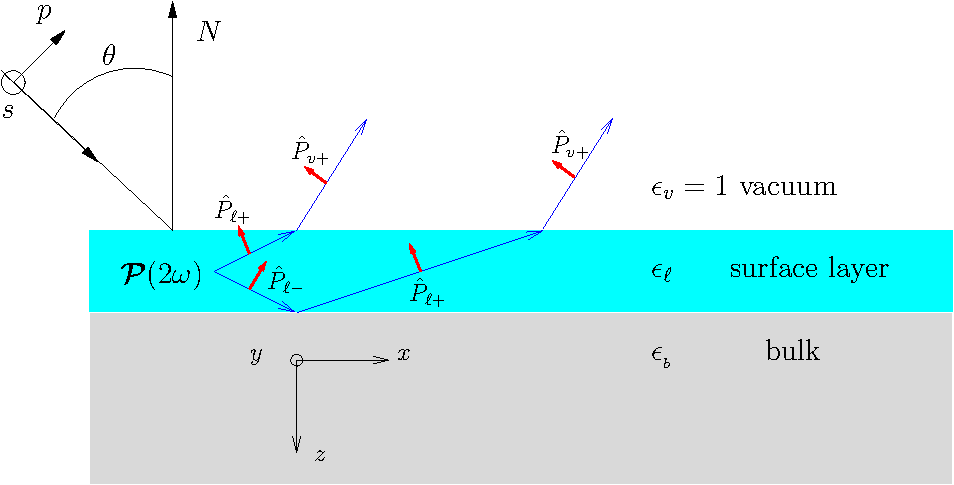
\includegraphics[width=0.7\textwidth]{figures/3layers.pdf}
\caption{Sketch of the three layer model for SHG. Vacuum is on top with
$\epsilon=1$, the layer with non-linear polarization
$\boldsymbol{\mathcal{P}}(2\omega)$ is characterized with
$\epsilon_{\ell(}\omega)$ and the bulk with $\epsilon_{b}(\omega)$. In the
dipolar approximation the bulk does not radiate SHG. The thin arrows are along
the direction of propagation, and the unit vectors for $p$-polarization are
denoted with thick arrows (capital letters denote SH components). The unit
vector for $s$-polarization points along $y$ (out of the page). $N$ is normal
to the surface, and $\theta$ is the angle of incidence for $p$ or $s$ input
polarization.\label{3layers}}
\end{figure}

We define the transmission, $\mathbf{T}$, and reflection, $\mathbf{R}$, tensors as,
\begin{equation}\label{r5}
\mathbf{T}_{\ell v}= \hat{\mathbf{s}}T_{s}^{\ell v}\hat{\mathbf{s}} + \hat{\mathbf{P}}_{v+}\tilde{T}_{p}^{\ell v} \hat{\mathbf{P}}_{\ell +},
\end{equation}
and
\begin{equation}\label{r6}
\mathbf{R}_{\ell b}= \hat{\mathbf{s}}R_{s}^{\ell b}\hat{\mathbf{s}} + \hat{\mathbf{P}}_{\ell +}R_{p}^{\ell b} \hat{\mathbf{P}}_{\ell -},
\end{equation}
where variables in capital letters are evaluated at the harmonic frequency
$2\omega$. Notice that since $\hat{\mathbf{s}}$ is independent of $\omega$, then
$\hat{\mathbf{s}}=\hat{\mathbf{s}}$. The Fresnel factors, $T_{i}$, $R_{i}$,
and $\tilde{T}_{p}$, for $i=s,p$ polarization, are evaluated at the appropriate
interface $\ell v$ or $\ell b$, and will be given below. The extra subscript
in $\hat{\mathbf{P}}$ denotes the corresponding dielectric function to be used in its
evaluation, i.e. $\epsilon_{v}=1$ for vacuum ($v$),
$\epsilon_{\ell}$ for the layer ($\ell$),
and $\epsilon_{b}$ for the bulk ($b$).
Therefore, the total radiated field at $2\omega$ is
\begin{align}\label{r7}
\mathbf{E}(2\omega) &=
E_{s}(2\omega)\left(\mathbf{T}_{\ell v} + \mathbf{T}_{\ell v}\cdot\mathbf{R}_{\ell b}\right)\cdot\hat{\mathbf{s}}\nonumber\\ 
&+ E_{p+}(2\omega)\mathbf{T}_{\ell v}\cdot\hat{\mathbf{P}}_{\ell +} + E_{p-}(2\omega)\mathbf{T}_{\ell v}\cdot\mathbf{R}_{\ell b}\cdot\hat{\mathbf{P}}_{\ell -}.
\end{align}
First, we develop an intermediate result,
\begin{align*}
\mathbf{T}_{\ell v}\cdot\mathbf{R}_{\ell b} &= (\hat{\mathbf{s}}T_{s}^{\ell v}\hat{\mathbf{s}} + \hat{\mathbf{P}}_{v+}\tilde{T}_{p}^{\ell v} \hat{\mathbf{P}}_{\ell +})\cdot(\hat{\mathbf{s}}R_{s}^{\ell b}\hat{\mathbf{s}} + \hat{\mathbf{P}}_{\ell +}R_{p}^{\ell b} \hat{\mathbf{P}}_{\ell -})\\
&= \hat{\mathbf{s}}T_{s}^{\ell v}R_{s}^{\ell b}\hat{\mathbf{s}} + \hat{\mathbf{P}}_{v+}\tilde{T}_{p}^{\ell v}R_{p}^{\ell b}\hat{\mathbf{P}}_{\ell -}
\end{align*}

We apply this result for the $E_{s}$ term in Eq. \eqref{r7},
\begin{align}\label{eq:es}
\left(\mathbf{T}_{\ell v} + \mathbf{T}_{\ell v}\cdot\mathbf{R}_{\ell b}\right)\cdot\hat{\mathbf{s}} = &\Bigl[\hat{\mathbf{s}}T_{s}^{\ell v}\hat{\mathbf{s}} + \hat{\mathbf{P}}_{v+}\tilde{T}_{p}^{\ell v} \hat{\mathbf{P}}_{\ell +}\nonumber\\
&+ \hat{\mathbf{s}}T_{s}^{\ell v}R_{s}^{\ell b}\hat{\mathbf{s}} + \hat{\mathbf{P}}_{v+}\tilde{T}_{p}^{\ell v}R_{p}^{\ell b}\hat{\mathbf{P}}_{\ell -} \Bigr]\cdot\hat{\mathbf{s}}\nonumber\\
= &\Bigl[\hat{\mathbf{s}}\tilde{T}_{s}^{\ell v}\bigl(1 + R_{s}^{\ell b})\hat{\mathbf{s}}\Bigr]\cdot\hat{\mathbf{s}}\nonumber\\
= &\hat{\mathbf{s}}\tilde{T}_{s}^{\ell v}\bigl(1 + R_{s}^{\ell b})
\end{align}
For $E_{p+}$,
\begin{align}\label{eq:ep+}
\mathbf{T}_{\ell v}\cdot\hat{\mathbf{P}}_{\ell +} &= (\hat{\mathbf{s}}T_{s}^{\ell v}\hat{\mathbf{s}} + \hat{\mathbf{P}}_{v+}\tilde{T}_{p}^{\ell v} \hat{\mathbf{P}}_{\ell +})\cdot\hat{\mathbf{P}}_{\ell +}\nonumber\\
&= \hat{\mathbf{P}}_{v+}\tilde{T}_{p}^{\ell v}
\end{align}
and lasty for For $E_{p-}$,
\begin{align}\label{eq:ep-}
\mathbf{T}_{\ell v}\cdot\mathbf{R}_{\ell b}\cdot\hat{\mathbf{P}}_{\ell -} &= (\hat{\mathbf{s}}T_{s}^{\ell v}R_{s}^{\ell b}\hat{\mathbf{s}} + \hat{\mathbf{P}}_{v+}\tilde{T}_{p}^{\ell v}R_{p}^{\ell b}\hat{\mathbf{P}}_{\ell -})\cdot\hat{\mathbf{P}}_{\ell -}\nonumber\\
&= \hat{\mathbf{P}}_{v+}\tilde{T}_{p}^{\ell v}R_{p}^{\ell b}
\end{align}
We replace Eqs. \eqref{eq:es}, \eqref{eq:ep+}, and \eqref{eq:ep-} into Eq. \eqref{r7},
\begin{align}\label{eq:e2w}
\mathbf{E}(2\omega) &=
E_{s}(2\omega)\Bigl[\hat{\mathbf{s}}\tilde{T}_{s}^{\ell v}\bigl(1 + R_{s}^{\ell b})\Bigr]\nonumber\\ 
&+ E_{p+}(2\omega)\Bigl[\hat{\mathbf{P}}_{v+}\tilde{T}_{p}^{\ell v}\Bigr] + E_{p-}(2\omega)\Bigl[\hat{\mathbf{P}}_{v+}\tilde{T}_{p}^{\ell v}R_{p}^{\ell b}\Bigr].
\end{align}

From Eqs. \eqref{eq:ep_miz} and \eqref{eq:es_miz}, we get that 
\begin{align}
E_{p\pm}(2\omega) &= \frac{4\pi i\omega}{c K_{z}}\hat{\mathbf{p}}_{\pm}\cdot\boldsymbol{\mathcal{P}},\label{eq:ep_miz2w}\\
E_{s}(2\omega) & = \frac{4\pi i\omega}{c K_{z}}\hat{\mathbf{s}}\cdot\boldsymbol{\mathcal{P}}\label{eq:es_miz2w},
\end{align}

Combining Eqs. \eqref{eq:ep_miz2w} and \eqref{eq:es_miz2w} into Eq. \eqref{eq:e2w}
\begin{align}
\mathbf{E}(2\omega) &= \frac{4\pi i\omega}{c K_{z}}\Bigl[\hat{\mathbf{s}}\tilde{T}_{s}^{\ell v}\bigl(1 + R_{s}^{\ell b})\hat{\mathbf{s}} + \hat{\mathbf{P}}_{v+}\tilde{T}_{p}^{\ell v}\hat{\mathbf{P}}_{\ell +} + \hat{\mathbf{P}}_{v+}\tilde{T}_{p}^{\ell v}R_{p}^{\ell b}\hat{\mathbf{P}}_{\ell -}\Bigr]\cdot\boldsymbol{\mathcal{P}}\\
&= \frac{4\pi i\omega}{c K_{z}}\Bigl[\hat{\mathbf{s}}\tilde{T}_{s}^{\ell v}\bigl(1 + R_{s}^{\ell b})\hat{\mathbf{s}} + \hat{\mathbf{P}}_{v+}\tilde{T}_{p}^{\ell v}\bigl(\hat{\mathbf{P}}_{\ell +} + R_{p}^{\ell b}\hat{\mathbf{P}}_{\ell -}\bigr)\Bigr]\cdot\boldsymbol{\mathcal{P}}\\
&= \frac{4\pi i\omega}{c K_{z}}\mathbf{H}\cdot\boldsymbol{\mathcal{P}}
\end{align}
which matches Eq. (31) from Ref. \cite{mendozaEPI04}. We establish some simple relationships between $T$ and $R$,
\begin{align}\label{r11}
T_{s}^{\ell v} &= \frac{K_{z\ell}}{\cos\theta}\,T_{s}^{v\ell},  \quad\quad
\tilde{T}_p^{\ell v} = \frac{\sqrt{\epsilon_{\ell}(2\omega)}K_{z\ell}}{\cos\theta}\,T^{v\ell}_{p},\\
1 - R^{\ell b}_{p} &= \frac{\epsilon_{\ell}(2\omega)K_{zb}}{K_{z\ell}}\,T_{p}^{\ell b}, \quad\quad 
1 + R_{p}^{\ell b} = \epsilon_{b}(2\omega)T_{p}^{\ell b},\label{r11d}
\end{align}

The magnitude of the radiated field is given by
$E(2\omega)=\hat{\mathbf{e}}^{out}\cdot\mathbf{E}(2\omega)$,
where $\hat{\mathbf{e}}^{out}$ is the polarization vector of the radiated field, for
instance $\hat{\mathbf{s}}$ or $\hat{\mathbf{P}}_{v+}$. Then we write
\begin{equation}\label{r10}
E(2\omega)=\frac{4\pi i\omega}{c}\mathbf{e}^{\,2\omega}\cdot\boldsymbol{\mathcal{P}},
\end{equation}
so
\begin{equation}
\mathbf{e}^{\,2\omega} = \frac{1}{K_{z\ell}}\hat{\mathbf{e}}^{out}\cdot\mathbf{H}
\end{equation}

We rewrite $\mathbf{H}$ using Eqs. \eqref{r11}, \eqref{r11d}, \eqref{eq:pvectors}, and \eqref{eq:svectors},
\begin{equation}
\mathbf{H} = \frac{K_{zl}}{\cos\theta}\left[\hat{\mathbf{s}}T_{s}^{v\ell}T_{s}^{\ell b}\hat{\mathbf{y}} - \hat{\mathbf{P}}_{v+}T_{p}^{v\ell}T_{p}^{\ell b}\bigl(\epsilon_{\ell}(2\omega)K_{zb}\hat{\mathbf{x}} + \epsilon_{b}(2\omega)\sin\theta\hat{\mathbf{z}}\bigr)\right],
\end{equation}
and so,
\begin{equation}
\mathbf{e}^{\,2\omega} = \frac{1}{\cos\theta}\hat{\mathbf{e}}^{out}\cdot\left[\hat{\mathbf{s}}T_{s}^{v\ell}T_{s}^{\ell b}\hat{\mathbf{y}} - \hat{\mathbf{P}}_{v+}T_{p}^{v\ell}T_{p}^{\ell b}\bigl(\epsilon_{\ell}(2\omega)K_{zb}\hat{\mathbf{x}} + \epsilon_{b}(2\omega)\sin\theta\hat{\mathbf{z}}\bigr)\right]
\end{equation}

We can now write our $2\omega$ radiated fields as,
\begin{align}
E_{s}(2\omega) &= \frac{4\pi i \omega}{c\cos\theta}\Bigl[T_{s}^{v\ell}T_{s}^{\ell b}\hat{\mathbf{y}}\Bigr]\cdot\boldsymbol{\mathcal{P}} = \frac{4\pi i \omega}{c\cos\theta}T_{s}^{v\ell}T_{s}^{\ell b}\chi_{yij}E_{i}(\omega)E_{j}(\omega),\label{eq:es2w}\\
E_{p}(2\omega) &= -\frac{4\pi i \omega}{c\cos\theta}T_{p}^{v\ell}T_{p}^{\ell b}\Bigl[\epsilon_{\ell}(2\omega)K_{zb}\hat{\mathbf{x}} + \epsilon_{b}(2\omega)\sin\theta\hat{\mathbf{z}}\Bigr]\cdot\boldsymbol{\mathcal{P}}\nonumber\\
&= -\frac{4\pi i \omega}{c\cos\theta}T_{p}^{v\ell}T_{p}^{\ell b}\Bigl[\epsilon_{\ell}(2\omega)K_{zb}\chi_{xij} + \epsilon_{b}(2\omega)\sin\theta\chi_{zij}\Bigr]E_{i}(\omega)E_{j}(\omega).\label{eq:ep2w}
\end{align}

As mentioned before $E_{i}(\omega)$ is the incident field given by the external
field properly screened; then we have
\begin{equation}\label{r15}
\mathbf{E}_{s}(\omega)=E_{o} t_{s}^{v\ell}\left(1 + r_{s}^{\ell b}\right)\hat{\mathbf{y}},
\end{equation}
and
\begin{equation}\label{r16}
\mathbf{E}_{p}(\omega)=E_{o}\left[
\tilde{t}_p^{v\ell}\left(1-r_p^{\ell b}\right)\cos\theta_\ell\hat{\mathbf{x}}
-\tilde{t}_p^{v\ell}\left(1+r_p^{\ell
b}\right)\sin\theta_\ell\hat{\mathbf{z}}\right],
 \end{equation}
where $E_{o}$ is the incoming amplitude and $\theta_\ell$ is the angle of
refraction in the layer. Notice that the transmitted and reflected fields in
the layer are taken into $\mathbf{E}_{s}$ and $\mathbf{E}_{p}$. From Eqs.
(\ref{r11}-\ref{r11d}) we get
\begin{equation}\label{r17}
\mathbf{E}_{s}(\omega)=E_{o} t_s^{v\ell}t_s^{\ell b}\hat{\mathbf{y}},
\end{equation}
and
\begin{equation}\label{r18}
\mathbf{E}_{p}(\omega)=E_{o} t_p^{v\ell}t_p^{\ell b}\left(\epsilon_{\ell}(\omega)k_{zb}\hat{\mathbf{x}} - \epsilon_{b}(\omega)\sin\theta\hat{\mathbf{z}}\right).
\end{equation}

Substituting Eqs. \eqref{r17} and \eqref{r18} into Eqs. \eqref{eq:es2w} and \eqref{eq:ep2w}, then finally substituting those into Eq. \eqref{final}, we get

\begin{equation}\label{r19}
 R_{iF}=\frac{32\pi^3\omega^2}{(n_oe)^2c^3\cos^2\theta}
\left|T_F^{v\ell}T_F^{\ell b}(t_i^{v\ell}t_i^{\ell b})^2\,r_{iF}\right|^2,
\end{equation}
where $i$ (lower case) stands for initial polarization and $F$ (upper case)
stands for final polarization, with
\begin{equation}\label{r20}
r_{iP}=\left(\epsilon_\ell(2\omega)K_{zb}\chi_{xjk} + \epsilon_b(2\omega)\sin\theta\chi_{zjk}\right)
E_j^i E_k^i,
\end{equation}
and
\begin{equation}\label{r21}
r_{iS}=\chi_{yjk}  E_j^i E_k^i,
\end{equation}
where from Eqs. (\ref{r17}-\ref{r18}),
\begin{subequations}\label{r23}
\begin{align}
\mathbf{E}^s&=\hat{\mathbf{y}}\\
\mathbf{E}^p&=\epsilon_\ell(\omega)k_{zb}\hat{\mathbf{x}}-\epsilon_b(\omega)\sin\theta\hat{\mathbf{z}}.
\end{align}
\end{subequations}
The $n_oe$ factor in Eq. (\ref{r19}), with $n_o$ the electronic density,
renders $\boldsymbol{\chi}$ dimensionless.
To complete the required formulas, we write down the Fresnel factors,
\begin{equation}\label{e.f1}
t_s^{v\ell}=\frac{2\cos\theta}{\cos\theta+k_{z\ell}},
\quad\quad
t_p^{v\ell}=\frac{2\cos\theta}{\epsilon_\ell(\omega)\cos\theta+k_{z\ell}},
\end{equation}
\begin{equation}\label{e.f3}
t_s^{\ell b}=\frac{2k_{z\ell}}{k_{z\ell}+k_{zb}},
\quad\quad
t_p^{\ell b}=\frac{2k_{z\ell}}{\epsilon_b(\omega)k_{z\ell}+\epsilon_s(\omega)k_{zb}},
\end{equation}
where the appropriate term $\sqrt{\epsilon(\omega)}$ from the usual definition of
$t_p$ has been taken out to give Eqs. (\ref{r20}) and
(\ref{r21}).

\section{Conclusions}\label{con}

We have presented a complete derivation of the required elements to
calculate in the independent particle approach (IPA) the microscopic  
surface second harmonic susceptibility tensor $\bfgchi^S(-2\go;\go,\go)$ 
using a layer-by-layer approach. We have done so for semiconductors using 
the length gauge for the coupling of the external electric field to the 
electron. 
%Also,
%we calculated the radiated efficiency $R$ within the three layer
%model. 
%The combination of $\boldsymbol{\chi}$ and $R$ allow us
%to study this fascinating surface optical phenomena.
